\documentclass[12pt, letterpaper]{scrartcl}

\usepackage{fullpage} % Set margins and place page numbers at bottom center
\usepackage[shortlabels]{enumitem} % Use a. in the enumerate
\usepackage{amsmath} % aligned equations
\usepackage{graphicx} % include figure
\usepackage{float} % usage of H for figure float
\usepackage{amssymb} % \varnothing
% \usepackage{subfigure}
\usepackage{xcolor} % color in math mode
\DeclareMathOperator*{\argmin}{argmin} % argmin

\begin{document}

% ### Header - start ###
    \begin{center}
    	\hrule
    	\vspace{0.4cm}
    	{\textbf { {\large Homework 5} \\ EE 513 --- Stochastic Systems Theory}}
    \end{center}
    { \textbf{Name:} Ali Zafari \hspace{\fill} \textbf{Student Number:} 800350381 \hspace{\fill} \textbf{Fall 2022} } \newline\hrule
% ### Header - end ###

\paragraph*{Problem 5.1} \hfill\\
\begin{enumerate}[((a))]
    \item
    First, since the variance of $X_i$ is one, then $\frac{(2a)^2}{12}=1$ and therefore $a=\sqrt{3}$.
    
    To find a general form for the distribution of $S_n$ we define a random variable $Y_i=\frac{X_i}{\sqrt{n}}$. And therefore $S_n=\sum Y_i$.
    
    As all $X_i$'s are iid, so are $Y_i$'s. Therefore the distribution of $S_n$ is the convolution of distribution of $Y_i$'s.
    
    \begin{align*}
        f_Y(y)=
        \begin{cases} 
            \frac{\sqrt{n}}{2a}  & \frac{-a}{\sqrt{n}} < y < \frac{a}{\sqrt{n}}\\
            0 & o.w.\\
        \end{cases}
    \end{align*}
    
    \begin{itemize}
        \item $S_2$
        \begin{align*}
            f_{S_2}(s)=f_Y(y)*f_Y(y)=
        \begin{cases} 
            \frac{1}{6}(s+\sqrt{6})   &{-\sqrt{6} < s < 0}\\
            \frac{1}{6}(-s+\sqrt{6})   &{0 < s < \sqrt{6}}\\
            0 & o.w.\\
        \end{cases}
        \end{align*}
        
        \item $S_3$
        \begin{align*}
            f_{S_3}(s)=f_Y(y)*f_Y(y)*f_Y(y)=
            \begin{cases} 
            \frac{(s+3)^2}{16}   &{-3 < s < -1}\\
            \frac{-s^2+3}{8}   &{-1 < s < 1}\\
            \frac{(-s+3)^2}{16}   &{1 < s < 3}\\
            0 & o.w.\\
        \end{cases}
        \end{align*}
    \end{itemize}
    \item
    By applying CLT, we have $\frac{S_n-\mathbb{E}[S_n]}{\sqrt{Var(S_n)}}\sim \mathcal{N}(0,1)$.
    \begin{align*}
        \mathbb{E}[S_n]&=0\\
        Var(S_n)&=\frac{1}{n}\times\sum Var(X_i)=1
    \end{align*}
    Therefore: $S_n\sim \mathcal{N}(0,1)$ as $n\rightarrow+\infty$.
    
    \item
    
    Following images showing pdf of sample mean compared with a Gaussian at each step.
    
    \begin{figure}[H]
    \centering
    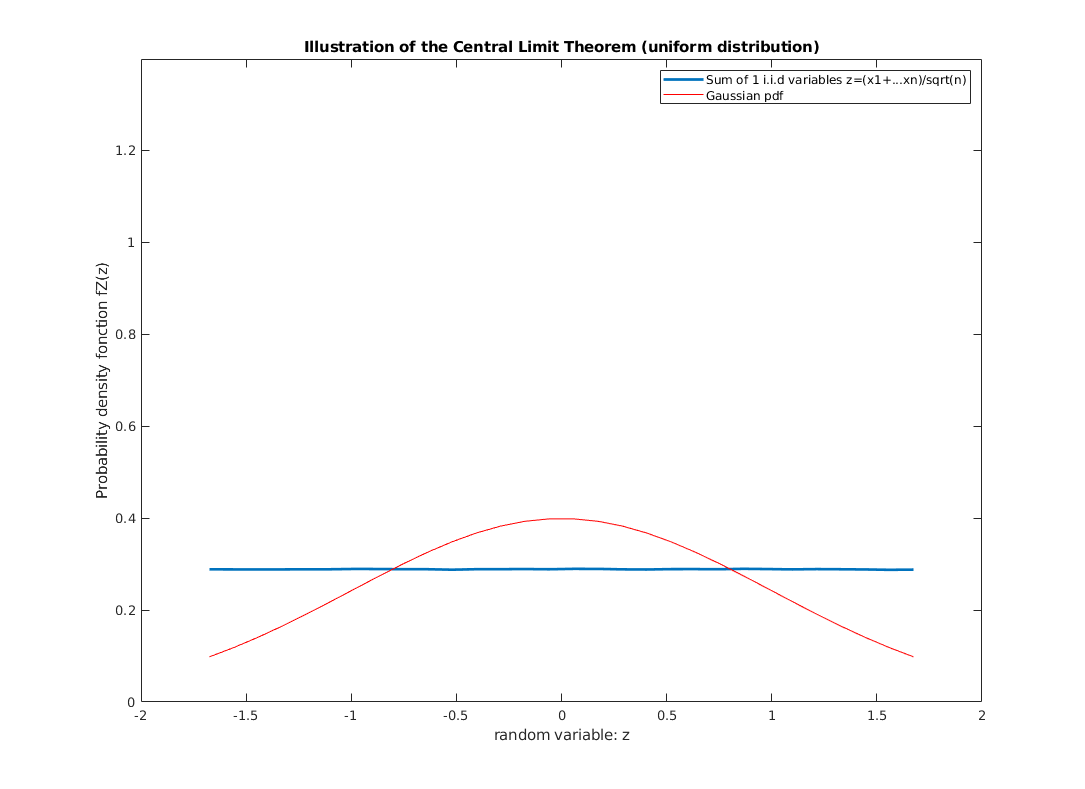
\includegraphics[width=0.9\textwidth]{hw5_figures/1.png}
    \end{figure}
    \begin{figure}[H]
    \centering
    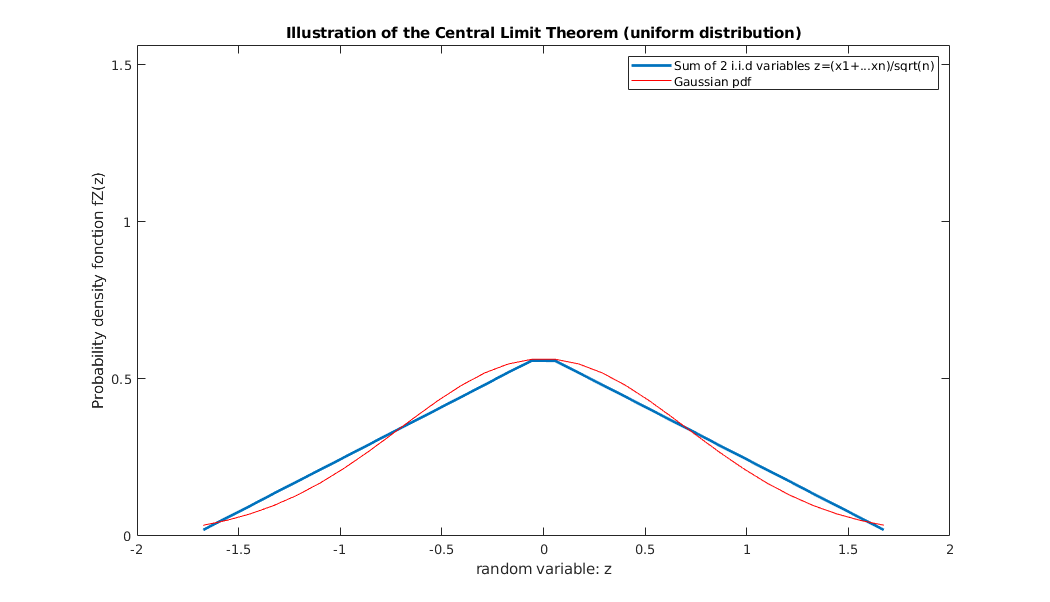
\includegraphics[width=0.9\textwidth]{hw5_figures/2.png}
    \end{figure}
    \begin{figure}[H]
    \centering
    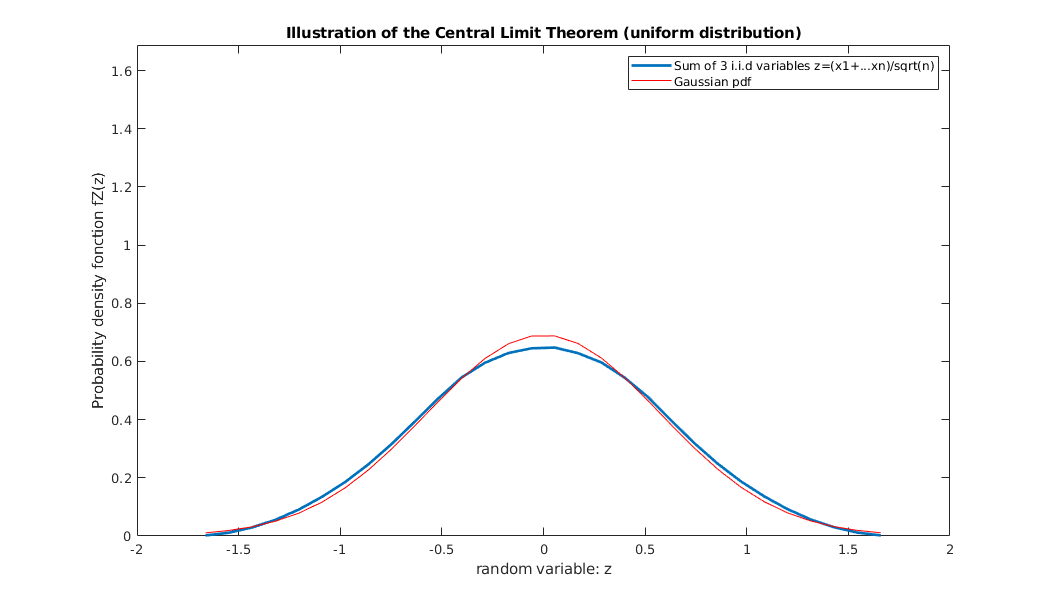
\includegraphics[width=0.9\textwidth]{hw5_figures/3.png}
    \end{figure}
    \begin{figure}[H]
    \centering
    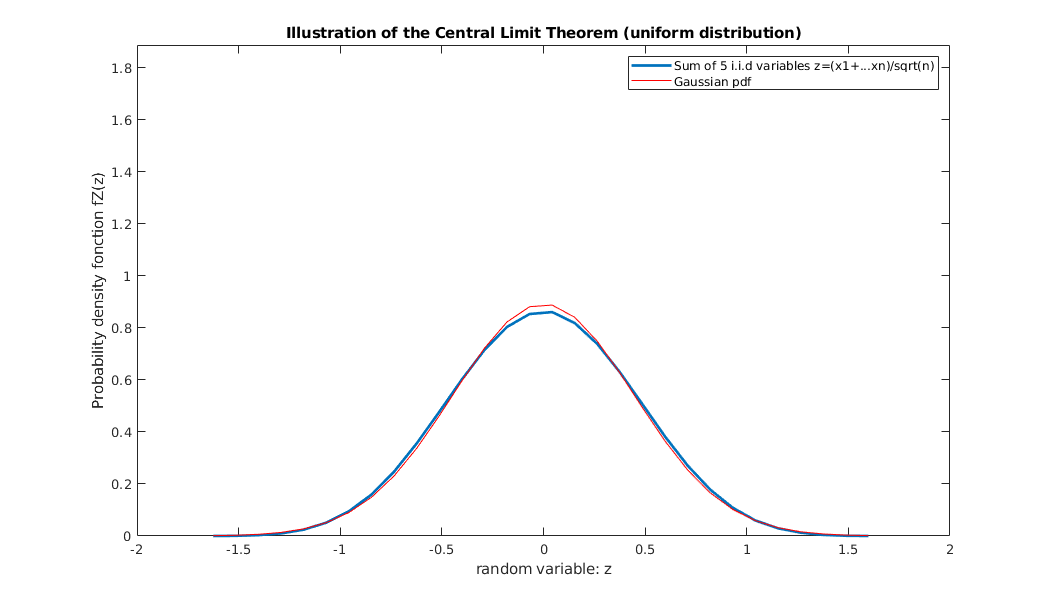
\includegraphics[width=0.9\textwidth]{hw5_figures/5.png}
    \end{figure}
    \begin{figure}[H]
    \centering
    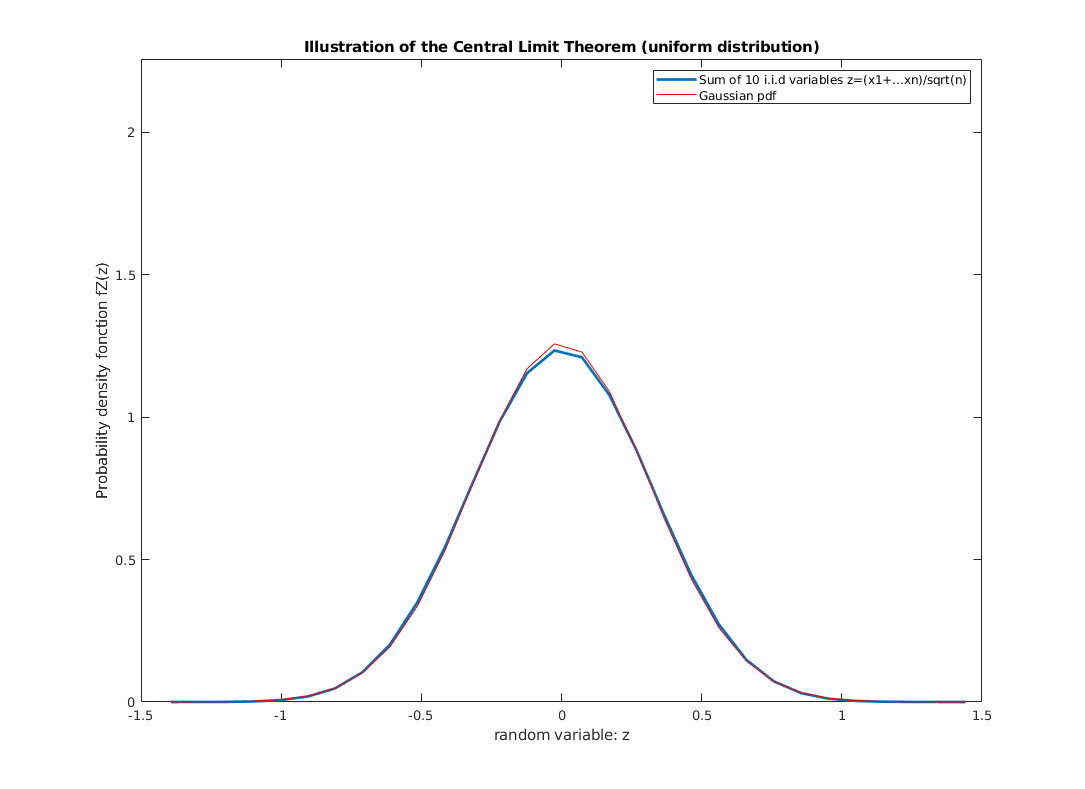
\includegraphics[width=0.9\textwidth]{hw5_figures/10.png}
    \end{figure}
    
    
\end{enumerate}
\hrule

\paragraph*{Problem 5.2} \hfill\\
\begin{enumerate}[((a))]
    \item For $Y=-\log(p(X))$:
    \begin{align*}
        \mathbb{E}_{y\sim P_Y(y)}[Y]&=\mathbb{E}_{x\sim P_X(x)}[-\log(p(x))]\\
        &=-\sum_{x\in \mathcal{X}}p(x)\log(p(x))\\
        &=\frac{1}{2}\times1+\frac{1}{4}\times2+\frac{1}{8}\times3+\frac{1}{16}\times4+\frac{1}{16}\times4\\
        &=1.875
    \end{align*}
    to find variance, we need $E_{y\sim P_Y(y)}[Y^2]=4.625-1.875^2=1.109375$:
    \begin{align*}
        \mathbb{E}_{y\sim P_Y(y)}[Y^2]&=\mathbb{E}_{x\sim P_X(x)}[\log^2(p(x))]\\
        &=\sum_{x\in \mathcal{X}}p(x)\log^2(p(x))\\
        &=\frac{1}{2}\times1+\frac{1}{4}\times4+\frac{1}{8}\times9+\frac{1}{16}\times16+\frac{1}{16}\times16\\
        &=4.625
    \end{align*}
    hence: $Var(Y)=\mathbb{E}[Y^2]-\mathbb{E}^2[Y]=4.625-1.875^2=1.109375$
    \item
    First we calculate the mean and variance of the arithmetic average of self-information ($X_i$'s are iid and $Y_i$'s are iid as well):
    \begin{align*}
        \mathbb{E}[S_n]&=n\times\frac{1}{n}\mathbb{E}[Y_1]=1.875\\
        Var(S_n)&=n\times\frac{1}{n^2}Var(Y_1)=\frac{1.109375}{n}
    \end{align*}
    Weak Law of Large Numbers (WLLN): as $n\rightarrow+\infty$ the difference between average self-information $S_n$ and its mean will converge \textbf{in probability} to zero.\\
    It can be proved by Chebyshev's inequality:
    \begin{align*}
        P(|S_n-\mathbb{E}[S_n]|>\epsilon)&\leq\frac{Var(S_n)}{\epsilon^2}=\frac{1.109375}{n\epsilon^2}
    \end{align*}
    hence, if $n\rightarrow+\infty$ then $P(|S_n-1.875|>\epsilon)\rightarrow0$.
\end{enumerate}
\hrule

\paragraph*{Problem 5.3} \hfill\\

\begin{enumerate}[((a))]
    \item 
    \begin{align*}
        \mathbb{E}[M_n]&=n\times\frac{1}{n}\mathbb{E}[X_i]=m\\
        Var(M_n)&=n\times\frac{1}{n^2} Var(X_i)=\frac{\sigma^2}{n}
    \end{align*}
    Since the expected valued of sample mean is equal to the mean, it is an \textbf{unbiased} estimator of mean of the random variable $X$.

    To check if the estimator of mean is consistent, we should see if it converges in probability to the true mean of the random variable $X$ or not. We exploit the \emph{Chebyshev}'s inequality to check this criterion.
    \begin{align*}
        P(|M_n-m|>\epsilon)&\leq\frac{Var(M_n)}{\epsilon^2}=\frac{\sigma^2}{n\epsilon^2}
    \end{align*}
    as we can see, when $n\rightarrow+\infty$ then $P(|M_n-m|>\epsilon)\rightarrow0$. So the estimator $M_n$ is \textbf{consistent}.
    \item
    \begin{align*}
        \mathbb{E}[V_n]&=\frac{1}{n-1}\sum_i\mathbb{E}[(X_i-M_n)^2]\\
        &=\frac{1}{n-1}\sum_i\mathbb{E}[X_i^2-2X_iM_n+M_n^2]\\
        &=\frac{1}{n-1}\sum_i\mathbb{E}[X_i^2]-2\mathbb{E}[X_iM_n]+\mathbb{E}[M_n^2]\\
        &=\frac{1}{n-1}\sum_i\mathbb{E}[X_i^2]-2\mathbb{E}[X_i\frac{X_1+\dots+X_i+\dots+X_n}{n}]+\mathbb{E}[M_n^2]\\
        &=\frac{1}{n-1}\sum_i\mathbb{E}[X_i^2]-\frac{2}{n}(\mathbb{E}[X_i^2] + (n-1)\mathbb{E}[X_iX_{j_{(j\neq i)}}])+\mathbb{E}[M_n^2]\\
        &=\frac{1}{n-1}\sum_i\mathbb{E}[X_i^2]-\frac{2}{n}(\mathbb{E}[X_i^2] + (n-1)\mathbb{E}[X_i]\mathbb{E}[X_{j_{(j\neq i)}}])+\mathbb{E}[M_n^2]\\
        &=\frac{1}{n-1}\sum_i\sigma^2+m^2-\frac{2}{n}(\sigma^2+m^2 + (n-1)m^2)+\frac{\sigma^2}{n}+m^2\\
        &=\frac{1}{n-1}\sum_i\frac{n\sigma^2+nm^2-2\sigma^2-2m^2+-2nm^2+2m^2+\sigma^2+nm^2}{n}\\
        &=\frac{1}{n-1}\sum_i\frac{(n-1)\sigma^2}{n}\\
        &=\frac{1}{n-1}n\frac{(n-1)\sigma^2}{n}\\
        &=\sigma^2
    \end{align*}
    
    \item
    \begin{align*}
        \mathbb{E}[V^{biased}_n]&=\frac{1}{n}\sum_i\mathbb{E}[(X_i-M_n)^2]\\
        &=\dots \text{Following the same steps above} \dots\\
        &=\frac{1}{n}\sum_i\frac{(n-1)\sigma^2}{n}\\
        &=\frac{1}{n}n\frac{(n-1)\sigma^2}{n}\\
        &=\frac{(n-1)}{n}\sigma^2
    \end{align*}
\end{enumerate}
 
\hrule

\paragraph*{Problem 5.4} \hfill\\
First, calculating the mean and variance of the sum of resistors, i.e. $S_4=\sum_{i=1}^4 R_i$:
\begin{align*}
    \mathbb{E}[S_4]&=4\times\mathbb{E}[R_1]=4\times500=2000\\
    Var(S_4)&=4\times Var(R_1)=4\times\frac{100^2}{12}=\frac{10000}{3}
\end{align*}
By applying CLT, we have $\frac{S_4-\mathbb{E}[S_4]}{\sqrt{Var(S_4)}}\sim \mathcal{N}(0,1)$. Therefore:
\begin{align*}
    P(1900\leq S_4\leq2100)&=P(\frac{1900-2000}{100/\sqrt{3}}\leq\frac{S_4-2000}{100/\sqrt{3}}\leq\frac{2100-2000}{100/\sqrt{3}})\\
    &=Q(-\sqrt{3})-Q(\sqrt{3})\\
    &=0.9167
\end{align*}
\hrule

\paragraph*{Problem 5.5} \hfill\\
\begin{enumerate}[((a))]
    \item For $S$ and $R$ to be jointly Gaussian, we should check that if their linear combination follows a Guassian distribution or not.
    To summarize:
    \begin{align*}
        S\sim \mathcal{N}(0,1)\\
        W\sim \mathcal{N}(0,1)\\
        R\sim \mathcal{N}(0,2)
    \end{align*}
    Let's assume random variable $P=aS+bR=(a+b)S+bW$. We calculate the characteristic function of $P$.
    \begin{align*}
        \mathbb{M}_{P}[jv]&=\mathbb{E}[e^{jv((a+b)S+bW)}]\\
        &=e^{\frac{-v^2(a+b)^2}{2}}.e^{\frac{-v^2(b)^2}{2}}\\
        &=e^{\frac{-v^2((a+b)^2+b^2)}{2}}
    \end{align*}
    Thus random variable $P$ is Gaussian with $\mathcal{N}(0,(a+b)^2+b^2)$. Then $S$ and $R$ are jointly Gaussian.
    
    \item
    By knowing that $\mathbb{E}[SR]-\mathbb{E}[R]\mathbb{E}[S] = \mathbb{E}[S^2+SW]=1+0=1$, 
    \begin{align*}
        K=
        \begin{bmatrix}
            Var(S) & \mathbb{E}[SR]-\mathbb{E}[R]\mathbb{E}[S] \\
            \mathbb{E}[SR]-\mathbb{E}[R]\mathbb{E}[S] & Var(R)
        \end{bmatrix}
        =
        \begin{bmatrix}
            1 & 1 \\
            1 & 2
        \end{bmatrix}
    \end{align*}
    
    \item
    The orthogonal transformation will be the eigenvectors of the covariance matrix. By using \emph{Matlab} we find the eigenvectors and eigenvalues of covariance matrix.
    \begin{align*}
        Q=
        \begin{bmatrix}
            -0.8507 & 0.5257 \\
            0.5257 & 0.8507
        \end{bmatrix}
    \end{align*}
    By using this transformation, the joint Gaussian will have the covariance matrix containing the eigenvalues of the original covariance matrix:
    \begin{align*}
        \Lambda=
        \begin{bmatrix}
            0.3820 & 0 \\
            0 & 2.6180
        \end{bmatrix}
    \end{align*}
\end{enumerate}
\hrule

\paragraph*{Problem 5.5} \hfill\\
\begin{enumerate}[((a))]
    \item Since, elements of vector $Y$ is linear combination of elements in $X$, distribution of $Y$ will be jointly Gaussian as well. Therefore by knowing the mean and covariance matrix of $Y$, its distribution will be fully characterized.
    \begin{align*}
        &\mathbb{E}[Y]=\mathbb{E}[C^{-1/2}X]=0\\
        &\mathbb{E}[YY^T]=\mathbb{E}[C^{-1/2}XX^TC^{{-1/2}^T}]=C^{-1/2}CC^{{-1/2}^T}=C^{-1/2}C^{1/2}C^{{1/2}^T}C^{{-1/2}^T}=I_{n\times n}
    \end{align*}
    Therefore $Y\sim\mathcal{N}(0, I_{n\times n})$.
    
    \item Let's define $Q\triangleq Y_k^2$, then we start with its CDF to find its PDF:
    \begin{align*}
        P(Y_k^2\leq q)=P(-\sqrt{q}\leq Y_k\leq \sqrt{q})=\int^{\sqrt{q}}_{-\sqrt{q}}\frac{1}{\sqrt{2\pi}}e^{-\frac{t^2}{2}}dt
    \end{align*}
    Using Leibniz integral rule, then we have a $\chi^2$ distribution with $1$ degree of freedom, as was expected from a square of normal random variable:
    \begin{align*}
        f_{Y_k^2}(y_k^2)=f_Q(q)=\frac{1}{2\sqrt{q}}\frac{1}{\sqrt{2\pi}}e^{-\frac{q}{2}}+\frac{1}{2\sqrt{q}}\frac{1}{\sqrt{2\pi}}e^{-\frac{q}{2}}=\frac{1}{\sqrt{2\pi q}}e^{-\frac{q}{2}}
    \end{align*}
    \item
    The sum of squares of $n$ independent Gaussian random variables (which is exactly the same as $V=\sum^n_{k=1}Y_k^2$), follows a $\chi^2$ distribution with $n$ degrees of freedom.
\end{enumerate}
\hrule

\end{document}

